\section{Analisi Target Utenti
}
Quando si crea un software, è importante ricordare che non è necessario soddisfare ogni singolo utente possibile, ma solo la categoria di utenti che usufruiranno del nostra sistema più frequentemente.\\
Questa decisione ci permette di concentrare la nostra analisi e ridurre funzioni che, al momento del rilascio del software al committente, sono superflue.\\
Uno strumento utile per fare questa analisi è la 
Persona, un modello di utente ideale che può essere basato su ricerche di mercato oppure da input dai committenti stessi.\\
\subsection*{Personas Individuate}
Per creare Personas è stato adottato un approccio basato su ipotesi e ricerche secondarie.\\
Abbiamo così definito il contesto, identificando il pubblico target, i loro obiettivi e le situazioni in cui potrebbero utilizzare il prodotto. Si possono utilizzare archetipi comuni del dominio di riferimento per immaginare utenti tipo, discutendo possibili bisogni, obiettivi e preferenze degli utenti.\\
Abbiamo creato le Personas a partire da una template predefinita e usando Figma per il design e l'aggiornamento di esse in corso d'opera.
\\

\begin{figure}[H]
\centering
\caption{Proprietario Agenzia immobiliare}
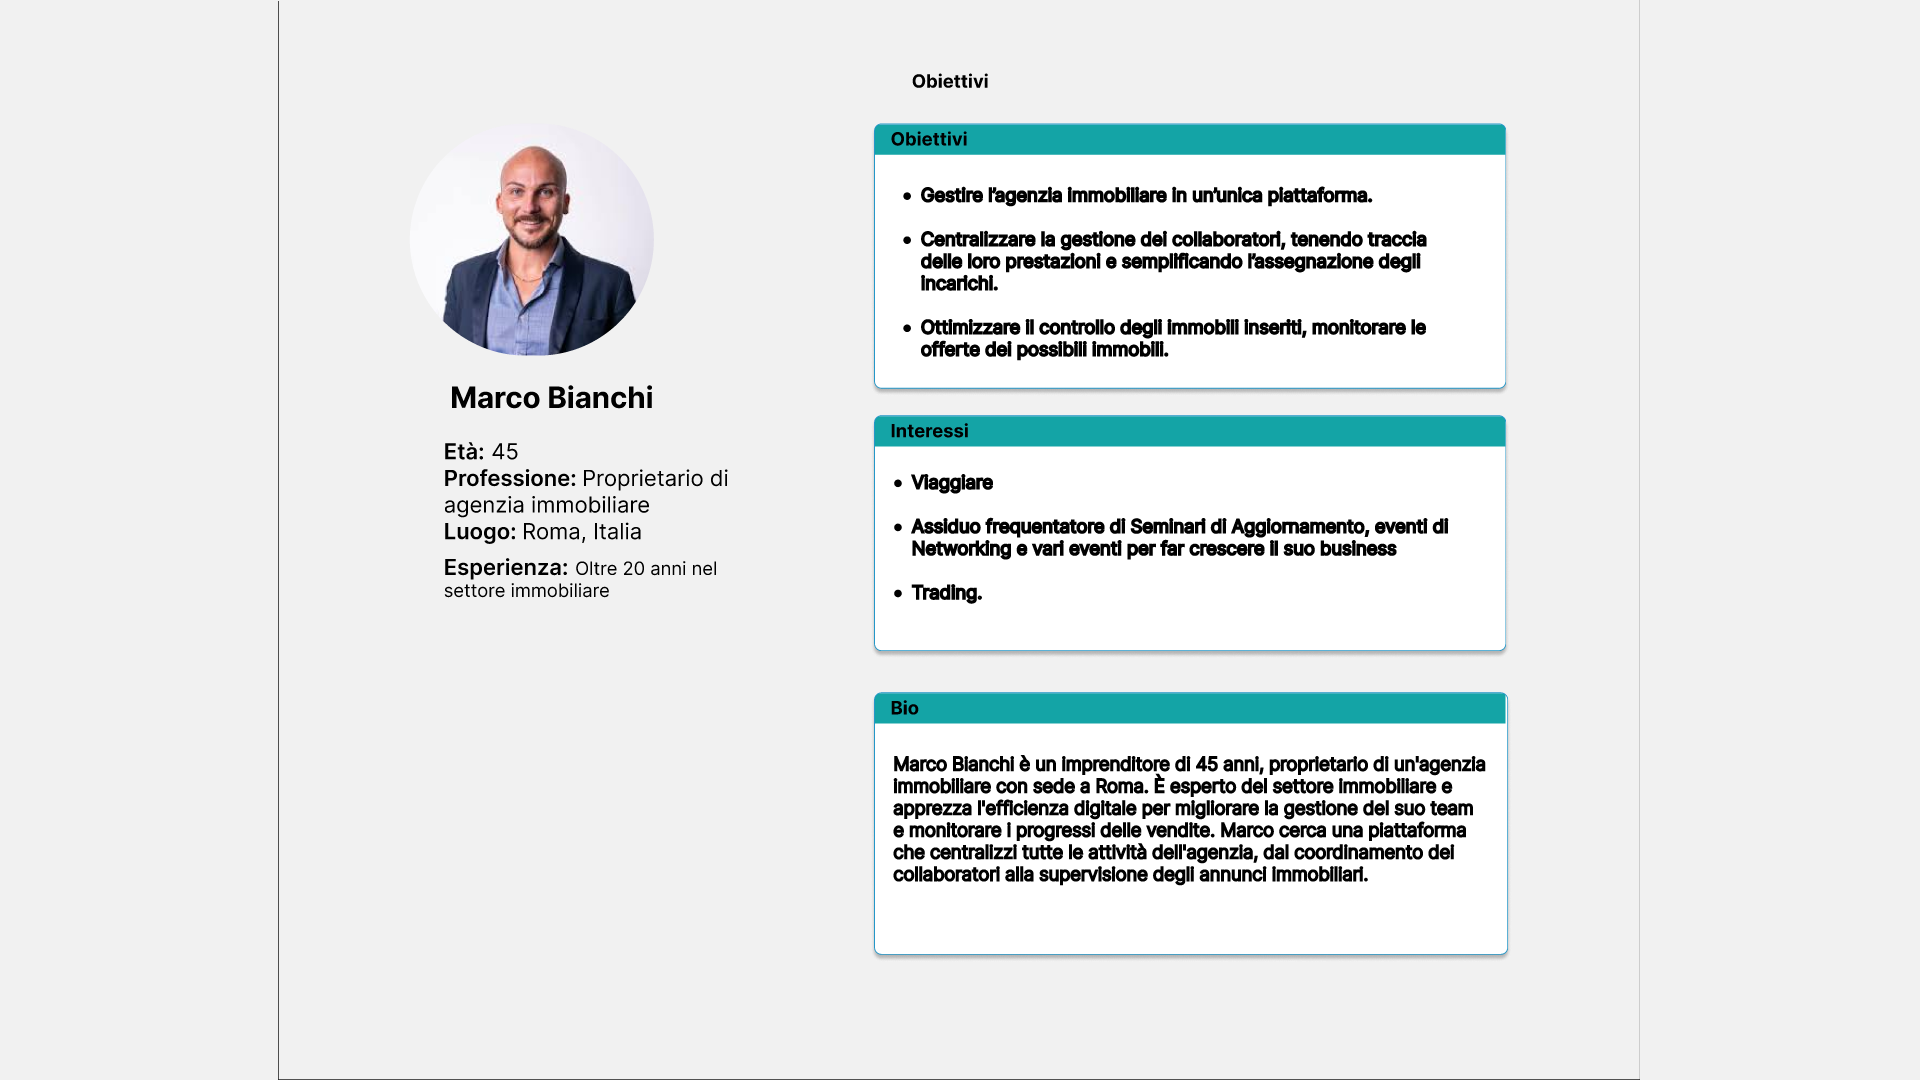
\includegraphics[width=1\textwidth]{{Immagini/Personas/Personas-Propretario di un agenzia immobiliare.png}}
\end{figure}

\begin{figure}[H]
\centering
\caption{Agente immobiliare}
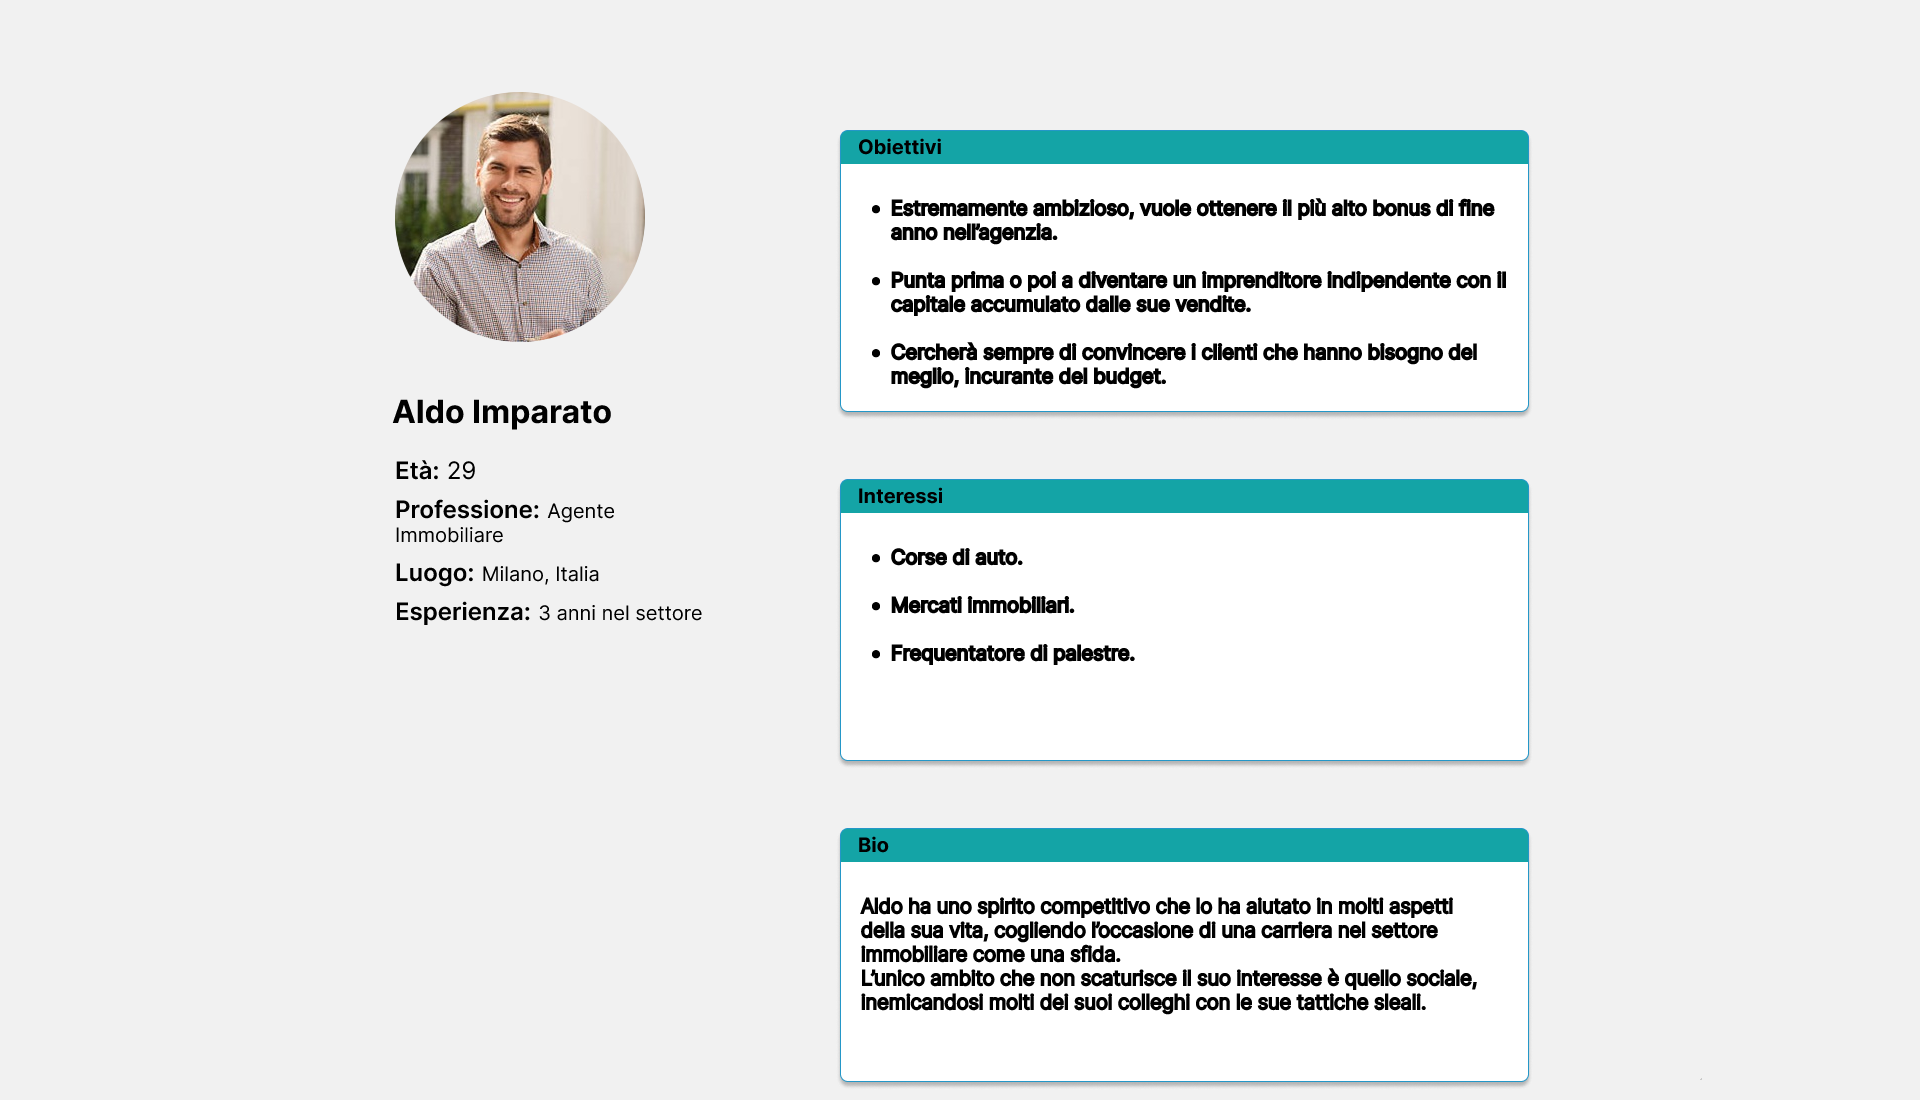
\includegraphics[width=1\textwidth]{{Immagini/Personas/Personas-Agente Immobiliare.png}}
\end{figure}

\begin{figure}[H]
\centering
\caption{Manager di azienda tecnologica}
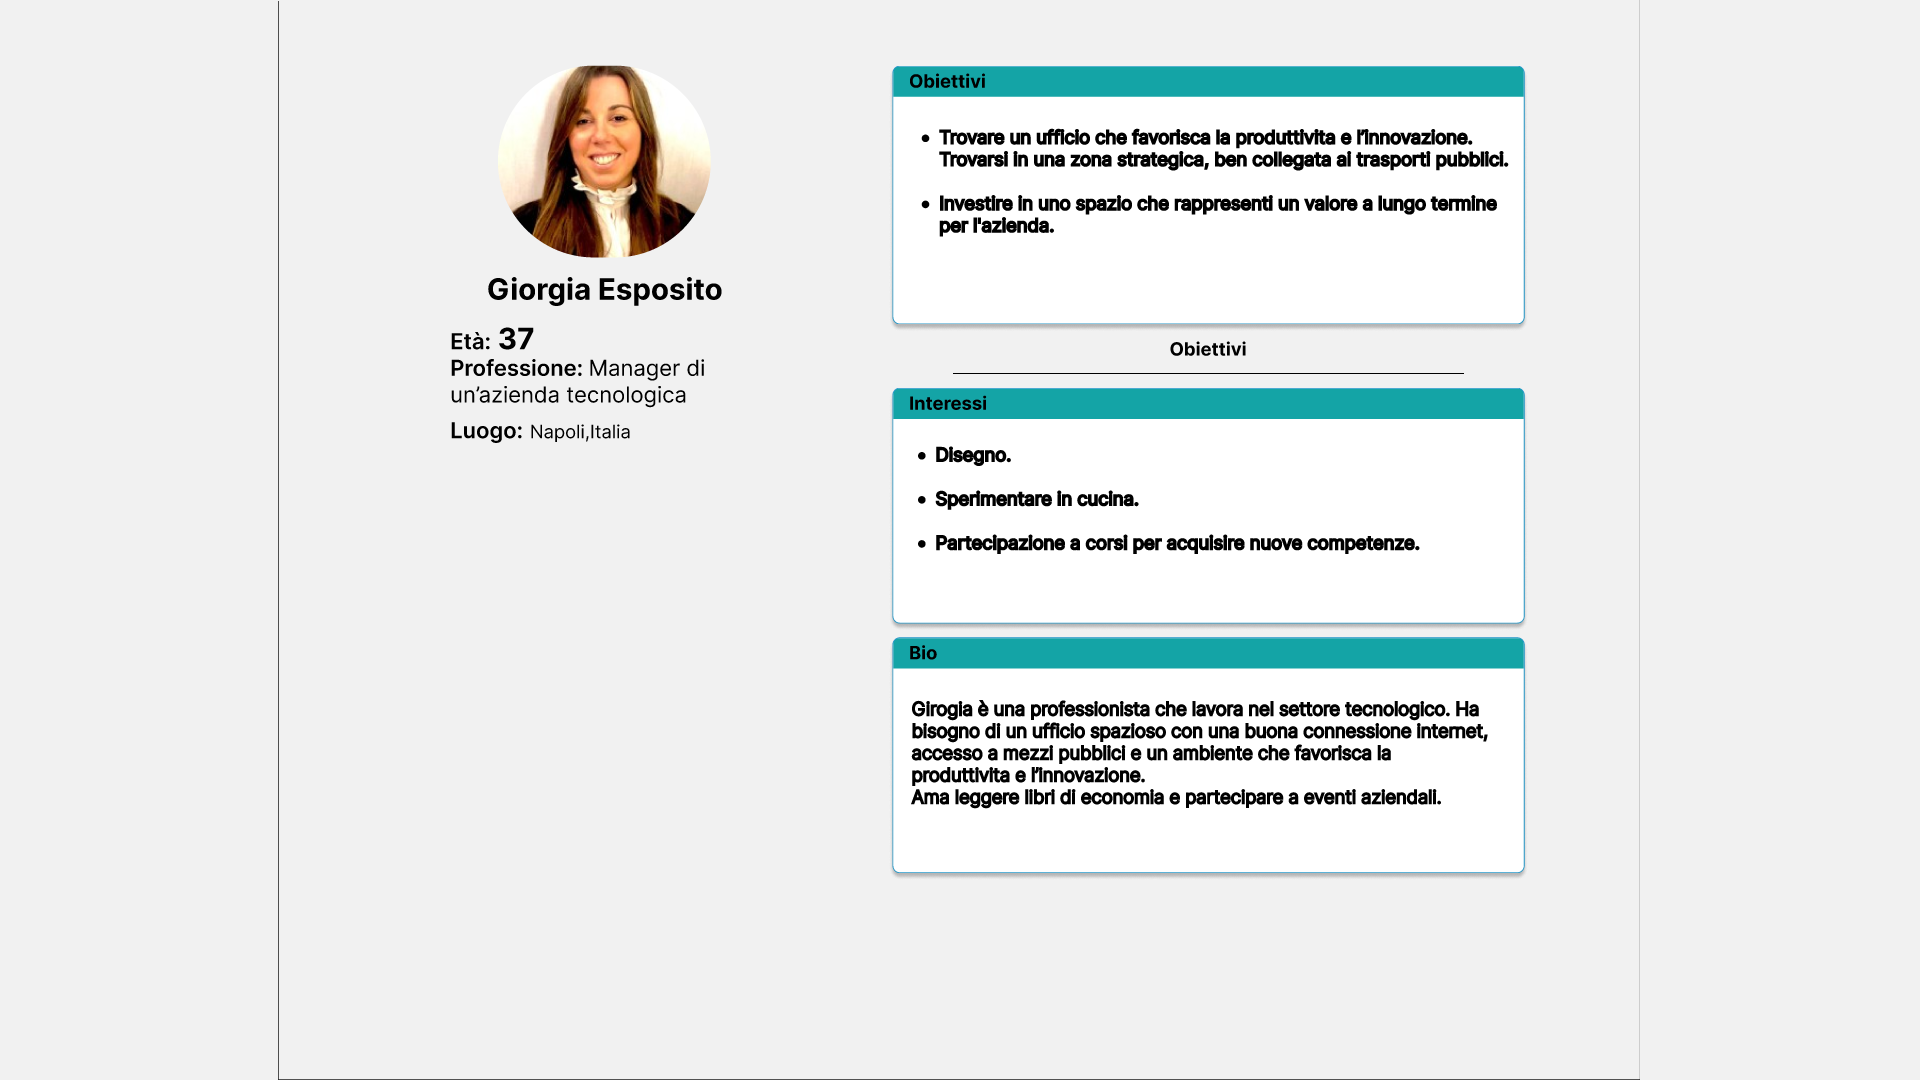
\includegraphics[width=1\textwidth]{Immagini/Personas/Personas-manager di azienda tecnologica.png}
\end{figure}

\begin{figure}[H]
\centering
\caption{Padre di famiglia}
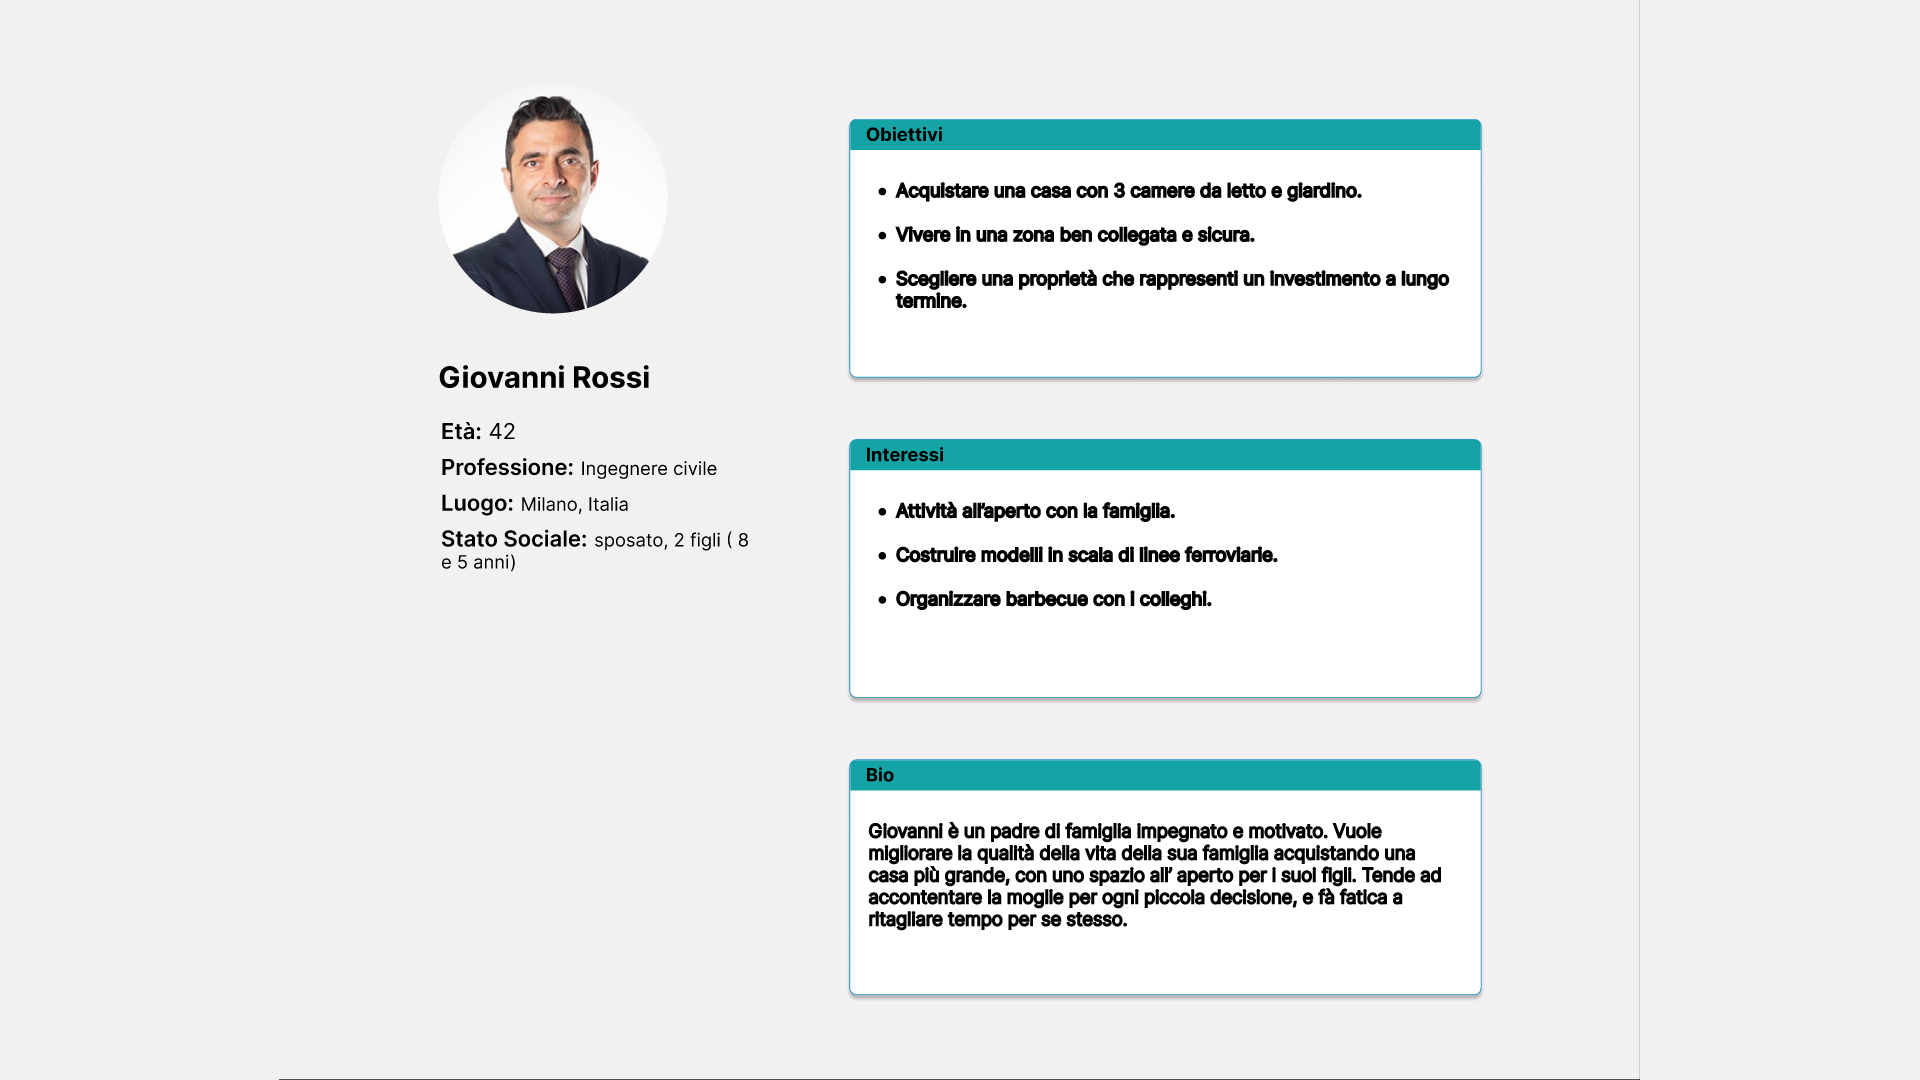
\includegraphics[width=1\textwidth]{Immagini/Personas/Personas-Padre di famiglia.png}
\end{figure}
\newpage
\subsection*{Tratti Caratteristici}
Analizzando queste Personas possiamo notare dei tratti che possiamo usare nella nostra applicazione:
\begin{itemize}
    \item  L'Agente- Aldo Imparato: questa categoria di utenti è parte dello staff dell'Agenzia immobiliare e quindi ha accesso al lato di amministrazione degli Immobili, e potrebbe volere una sezione nella sa pagina personale che gli mostra tutti gli Immobili a suo carico.
    \item  Il Padre di Famiglia - Giovanni Rossi: l'archetipo che incarna il Utente medio che ha vaghe idee su cosa vuole e si affida all'agente immobiliare. Dobbiamo quindi tener conto che le informazioni visibili a questo tipo di utenti deve essere chiara e concisa, come ad esempio le etichette che indicando punti di interesse come parchi e scuole.
    \item Il Manager di Azienda Tecnologica - Giorgia Esposito: l'utente che sta cercando qualcosa di ben definito, ma l'agenzia non offre Immobili con le caratteristiche cercate. Per questo tipo di persone offriremo un servizio di iscrizione ai tag di interesse per ricevere notifiche quando un immobile che rispecchia tali desideri viene messo in vendita.
    \item Il Proprietario dell'Agenzia Immobiliare - Marco Bianchi: gli amministratori del sistema che gestiscono dipendenti e il catalogo di Immobili, questo tipo di utente deve gestire multipli dati personali e sensibili. Quando crea un Agente o Amministratore, le nuove informazioni verranno generate dal sistema e inviate tramite un servizio di posta elettronica.
\end{itemize}
\newpage